\documentclass{article}

\usepackage{amsthm, amsfonts, amsmath, amssymb}
\usepackage{graphicx}
\usepackage{fullpage}
\usepackage{float}
\usepackage{hyperref}

\newtheorem{lemma}{Lemma}
\newtheorem{theorem}{Theorem}
\newtheorem{corollary}{Corollary}
\newtheorem{conjecture}{Conjecture}
\newtheorem{definition}{Definition}

\setlength{\parindent}{0em}

\renewcommand{\O}{\mathcal{O}}
\newcommand{\N}{\mathbb{N}}
\newcommand{\xor}{\oplus}

\begin{document}
	\title{The Rank Deficiency of Certain Sized \textit{Lights Out} Boards}
	\author{William Boyles}
	\date{\today}
	\maketitle
	
	\section{Intro Lemmas}
	Let $f(n,x)$ be the Chebyshev polynomial over $GF(2)$ that we defined previously.
	Recall that the rank deficiency of an $n \times n$ \textit{Lights Out} board, $d(n)$, is the degree of $\gcd(f(n,x), f(n,x+1))$.
	Let $g: \N \to \N$ where $g(k) = 2^{k+1} + 2^{k-1} - 1$.

	\begin{lemma}
		\label{conj1}
		Let $k \in \N$.
		Then
		\begin{equation*}
			f(g(k), x) = x^{2^{k-1}-1}\left(x^{2^{k+1}}+x^{2^k}+1\right).
		\end{equation*}
	\end{lemma}
	\begin{proof}
		Recall how we determine the coefficients of $f(n,x)$ using the parity of binomial coefficients.
		First, we need to find a value $K = 2^{k} - 1$ where $k$ is the smallest integer $K \geq n$.
		Second, we find $S = 2(K - n)$.
		Finally, we find that the $i$th coefficient is 1 if and only if $\binom{2i+S}{S+i}$ is odd. Equivalently, it's 1 if and only if $i \texttt{ \& } S+i$ is zero.
		$K = 2^{k+2} - 1$ for $g(k) = 2^{k+1} + 2^{k-1} - 1$.
		So,
		\begin{align*}
			S &= 2(K - g(k)) \\
			&= 2\left((2^{k+2}-1) - (2^{k+1} + 2^{k-1} - 1)\right) \\
			&= 2\left(2^{k+2} - 2^{k+1} - 2^{k-1}\right) \\
			&= 2\left(8\cdot2^{k-1} - 4\cdot2^{k-1} - 2^{k-1}\right) \\
			&= 2\left(3\cdot2^{k-1}\right) \\
			&= 3\cdot2^k.
		\end{align*}
		In binary this is $S = 11\underbrace{0 \dots 0}_{k}$. \\
		
		Let's think about what happens when we do $i \texttt{ \& } S + i$ for various values of $i$.
		\begin{itemize}
			\item
				In $i = 0$, we see that the left side of the \texttt{\&} is 0, so the entire result is 0. Therefore, the leading coefficient is a 1, as desired.
			\item
				In $i = 1 \dots 2^k - 1$, the trailing $k$ 0's in $S$ will match whatever is in $i$'s binary representation in $S + i$.
				So, the result of the \texttt{\&} will be nonzero.
				Therefore, there will be $2^k - 1$ 0 coefficients following the leading 1, as desired.
			\item
				In $i = 2^k$, $S + i = 100\underbrace{0 \dots 0}_{k}$.
				So, the \texttt{\&} will result in a 0, meaning we get a coefficient of 1, as desired.
			\item
				In $i = 2^k + 1 \dots 2^{k+1} - 1$, we see a combination of the previous two cases.
				We can write $i = 2^k + j$, where $1 \leq j \leq 2^{k} - 1$.
				As we saw in the previous case, $S + 2^k = 100\underbrace{0 \dots 0}_{k}$ in binary.
				As in two cases ago, the trailing $k$ 0's in $S + 2^k$ will match whatever is in $j$'s binary representation in $S + 2^k + j$.
				So, the result of the \texttt{\&} operation will be nonzero.
				Therefore, the second 1 coefficient will be followed by $2^k - 1$ 0 coefficients, as desired.
			\item
				In $i = 2^{k+1}$, $S + i = 101\underbrace{0 \dots 0}_{k}$.
				Since $i$ does not have a $2^k$ or a $2^{k+2}$ in its binary representation, $i \texttt{ \& } S+i \texttt{ == } 0$.
				So, we get a coefficient of 1, as desired.
			\item
				In $i = 2^{k+1} + 1 \dots 2^{k+1} + 2^{k-1} - 1$, we again see a combination of previous cases.
				We can write $i = 2^{k+1} + j$, where $1 \leq j \leq 2^{k-1} - 1$.
				As we saw in the previous case, $S + 2^{k+1} = 101\underbrace{0 \dots 0}_{k}$.
				As in two cases ago, the trailing $k$ 0's in $S + 2^{k+1}$ will match whatever is in $j$'s binary representation in $S + 2^{k+1} + j$.
				So, the result of the \texttt{\&} operation will be nonzero.
				Therefore, the third 1 coefficient will be floowed by $2^{k-1} - 1$ 0 coefficients, as desired.
		\end{itemize}	
	\end{proof}

	\begin{lemma}
		\label{conj2}
		Let $k \in \N$.
		Then
		\begin{equation*}
			f(g(k), x+1) = \left(x^{2^{k+1}}+x^{2^k}+1\right)\left(x^{2^{k-1}-1}+\dots+1\right).
		\end{equation*}
	\end{lemma}
	\begin{proof}
		In lemma \ref{conj1}, we showed that
		\begin{equation*}
			f(g(k),x) = \left(x^{2^{k-1}-1}\right)\left(x^{2^{k+1}} + x^{2^{k}} + 1\right).
		\end{equation*}
		Substituting $x+1$ for $x$ and using mod 2 arithmetic (i.e. $(a+b)^c = a^c + b^c$ where $c$ is a power of 2; $1 = -1$),
		\begin{align*}
			f(g(x), x+1) &= \left((x+1)^{2^{k-1}-1}\right)\left((x+1)^{2^{k+1}} + (x+1)^{2^k} + 1\right) \\
			&= \left(x^{2^{k-1}}+1\right)\frac{1}{x+1}\left(x^{2^{k+1}} + 1 + x^{2^k} + 1 + 1\right) \\
			&= \left(x^{2^{k+1}} + x^{2^k} + 1\right)\frac{x^{2^{k-1}}-1}{x-1} \\
			&= \left(x^{2^{k+1}} + x^{2^k} + 1\right)\left(x^{2^{k-1}-1} + x^{2^{k-1}-2} + \dots + 1\right).
		\end{align*}
	\end{proof}
	
	\section{Main Result}
	Now that we have lemmas \ref{conj1} and \ref{conj2}, we can prove our main result.
	\begin{theorem}
		Let $k \in \N$.
		Then
		\begin{equation*}
			\gcd\left(f(g(k),x),f(g(k),x+1)\right) = x^{2^{k+1}} + x^{2^k} + 1.
		\end{equation*}
	\end{theorem}
	\begin{proof}
		We can see from lemmas 
		\ref{conj1} and \ref{conj2} that the desired gcd is a common factor of both polynomials.
		So, we just need to show that over $GF(2)$ that the remaining factors of both polynomials have no common factors.
		This result is easily verified by a computer.
		
		\begin{figure}[H]
			\centering
			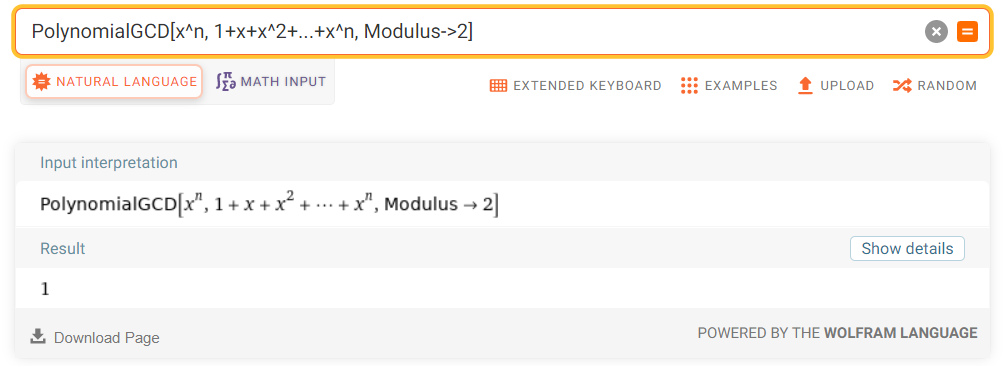
\includegraphics[width=.8\textwidth]{wolfram_result.png}
			\caption{\href{https://www.wolframalpha.com/input/?i=PolynomialGCD\%5Bx\%5En\%2C+1\%2Bx\%2Bx\%5E2\%2B...\%2Bx\%5En\%2C+Modulus-\%3E2\%5D}{Wolfram|Alpha: PolynomialGCD[$x^n, 1+x+x^2+...+x^n$, Modulus$\to$2]}}
		\end{figure}
	\end{proof}

	\begin{corollary}
		A \textit{Lights Out} board of size $g(k) \times g(k)$ will have nullity $2^{k+1}$.
	\end{corollary}
	
	\section{Concluding Conjectures}
	\begin{conjecture}
		\label{conj3}
		Let $h: \N \to \N$ where
		\begin{equation*}
			h(n) = \max \{g(m) \mid m \in \N, g(m) \leq n\}.
		\end{equation*}
		Then for all $n \in \N$,
		\begin{equation*}
			\max \{d(m) \mid 1 \leq m \leq n\} = d(h(n)).
		\end{equation*}
	\end{conjecture}
	In other words, if we list the board sizes and their rank deficiencies, noting each time we encounter a rank deficiency higher than any other we've seen before, we will have noted exactly the board sizes described by $g$. \\
	
	Unfortunately, this isn't always true
	\begin{proof}[Disproof.]
		Notice that for $n=30$,
		\begin{align*}
			h(30) &= \max\{g(m) \mid n \in \N, g(m) \leq 30\}
			&= \max\{g(1), g(2), g(3)\} \\
			&= \max\{4, 9, 19\} \\
			&= 19,
		\end{align*}
		and
		\begin{align*}
			\max\{d(m) \mid 1 \leq m \leq 30\} &= \max\{d(1),d(2),\dots,d(29),d(30)\} \\
			&= \max\{0,0,\dots,10,20\} \\
			&= 20.
		\end{align*}
		However,
		\begin{equation*}
			20 \neq d(19) = 16.
		\end{equation*}
	\end{proof}

	\begin{conjecture}
		For all $n \in \N$, $d(n) \leq n$, and $d(n) = n$ only when $n=4$.
	\end{conjecture}
	This conjecture may be proven by others using different methods.
\end{document}